\documentclass[12pt, titlepage]{article}
\usepackage[shortlabels]{enumitem}
\usepackage{comment}
\usepackage{booktabs}
\usepackage{tabularx}
\usepackage{hyperref}
\usepackage{float}
\usepackage{soul}
\usepackage{changepage}
\usepackage{graphicx}
\hypersetup{
    colorlinks,
    citecolor=blue,
    filecolor=black,
    linkcolor=red,
    urlcolor=blue
}
\usepackage[round]{natbib}
\usepackage[dvipsnames]{xcolor}

%% Comments

\usepackage{color}

\newif\ifcomments\commentstrue %displays comments
%\newif\ifcomments\commentsfalse %so that comments do not display

\ifcomments
\newcommand{\authornote}[3]{\textcolor{#1}{[#3 ---#2]}}
\newcommand{\todo}[1]{\textcolor{red}{[TODO: #1]}}
\else
\newcommand{\authornote}[3]{}
\newcommand{\todo}[1]{}
\fi

\newcommand{\wss}[1]{\authornote{blue}{SS}{#1}} 
\newcommand{\plt}[1]{\authornote{magenta}{TPLT}{#1}} %For explanation of the template
\newcommand{\an}[1]{\authornote{cyan}{Author}{#1}}

%% Common Parts

\newcommand{\progname}{ProgName} % PUT YOUR PROGRAM NAME HERE
\newcommand{\authname}{Team \#, Team Name
\\ Student 1 name
\\ Student 2 name
\\ Student 3 name
\\ Student 4 name} % AUTHOR NAMES                  

\usepackage{hyperref}
    \hypersetup{colorlinks=true, linkcolor=blue, citecolor=blue, filecolor=blue,
                urlcolor=blue, unicode=false}
    \urlstyle{same}
                                


\begin{document}

\title{System Verification and Validation Plan for \progname{}} 
\author{\authname}
\date{\today}
	
\maketitle

\pagenumbering{roman}

\begin{table}[H]
  \caption{\bf Revision History}
  \begin{tabularx}{\textwidth}{p{2.5cm}p{2.5cm}X}
  \toprule {\bf Date} & {\bf Developer} & {\bf Notes/Changes}\\
  \midrule
  Oct 31, 2022 & Timothy Chen & Added to 5.2, 5.3, 7.2\\
  Oct 31, 2022 & Edwin Do & Added section 4 for V\&V Plan\\
  Nov 1, 2022 & Abdul Nour Seddiki & Added to 5.1, 5.3\\
  Nov 2, 2022 & Joseph Braun & Added Section 3\\
  Nov 2, 2022 & Edwin Do & Added more content to section 4 \\
  Mar 4, 2023 & Edwin Do & Revised tests for non functional requirements\\
  Mar 4, 2023 & Timothy Chen & Revised Usability and Performance NFR test\\
  Mar 6, 2023 & Abdul Nour Seddiki & Revised tests for Functional Requirements \& fixed formatting\\
  Mar 8, 2023 & Edwin Do, Timothy Chen & Further revision of tests for non functional requirements\\
  Mar 8, 2023 & Tyler Magarelli & Updated user experience survey for section 6.2\\
  \bottomrule
  \end{tabularx}
  \end{table}
  

\newpage

\tableofcontents

\listoftables
%\wss{Remove this section if it isn't needed}

%\listoffigures
%\wss{Remove this section if it isn't needed}

\newpage

\section{Symbols, Abbreviations and Acronyms}

\renewcommand{\arraystretch}{1.2}
\begin{tabular}{l l} 
  \toprule		
  \textbf{symbol} & \textbf{description}\\
  \midrule 
  T & Test\\
  SRS & Software Requirements Specifications \\
  VS & Visual Studio\\
  UWP & Universal Windows Platform\\
  MIN\_USER\_ACCEPT\_RATE & 90\% - minimum acceptance rate\\
  TARGET\_TIME & 60 seconds \\
  INTERACT\_TIME & 5 seconds \\
  MAX\_MISTAKE & 2 \\
  MAX\_SIZE & 8GB \\ 
  MIN\_UPTIME & 30 minutes \\ 
  MIN\_SAMPLE\_RATE & 60 samples per second\\
  TIME\_ACCEPTED & 1 second \\
  ACCEPTED\_SIGFIG & 3 decimals \\
  \bottomrule
\end{tabular}\\

\wss{symbols, abbreviations or acronyms -- you can simply reference the SRS
  \citep{SRS} tables, if appropriate}

\newpage

\pagenumbering{arabic}

\section{General Information}

\subsection{Summary}

The purpose of this document is to provide a detailed plan for the testing of our system. This will include:
\begin{itemize}
  \item Verification and Validation Plan
  \item System Test Description
  \item Unit Test Description
\end{itemize}

\subsection{Objectives}

The objectives of testing are to ensure that all functional and non-functional requirements of the system are being met. It is important to include both unit tests as well as system tests, as issues may arise when components are connected together in the system. 

\subsection{Relevant Documentation}

Relevant documentation includes:
\begin{itemize}
  \item SRS
  \item MIS
  \item MG
\end{itemize}

\section{Plan}
% RUBRIC
% 'Team member's roles for testing are clear;  
% This may involve switching roles between verification tasks 
% (say between SRS verification, hardware verification, and code verification).  
% Clear, specific and feasible plan for SRS verification; 
% Clear specific and feasible plan for Design verification; 
% Clear specific and feasible plan for implementation verification.  
% Automated testing and verification tools are specific.  
% Software validation plan is clear, specific and feasible.

% \wss{Introduce this section.   You can provide a roadmap of the sections to
%   come.}

  In this section of planning, it will outline our approaches to cover the requirements 
  outlined in various areas such as the SRS document, Hazard analysis document, our implementation and design. 
  Tools that will be used for automated unit testing and linting will also be introduced.\\

  The following topics will be covered:

  \begin{itemize}
    \item The verification and validation team along with their respective responsibilities
    \item Our approach towards the SRS Verification plan
    \item Our approach towards the Design Verification plan
    \item Implementation verification plan
    \item Any testing and verification tools we plan to use
  \end{itemize}


\subsection{Verification and Validation Team}

% \wss{You, your classmates and the course instructor.  Maybe your supervisor.
%   You shoud do more than list names.  You should say what each person's role is
%   for the project.  A table is a good way to summarize this information.}

  Below is a table outlining the members of the Verification and Validation team along with their respective responsibilities.
  Note that the listed responsibilities are only used as a guideline, responsibilities can shift between team members on a as-per-needed basis.

  \begin{table}[H]
    \centering
    \caption{Team and Responsibilities}
    \label{my-label}
    \begin{tabular}{|c|c|c|}
      \hline
      \textbf{Team Member} & \textbf{Role Name} & \textbf{Responsibilities}   \\ \hline
      Edwin Do & 
      \begin{tabular}{@{}c@{}}Software and SRS Tester\end{tabular} & 
      \begin{tabular}{@{}c@{}}Ensures that all requirements are valid \\ 
        and verified under the scope of software \\
        capabilities in this project and the SRS\end{tabular} \\ \hline
      
      Timothy Chen & 
      \begin{tabular}{@{}c@{}}Software Tester\end{tabular} & 
      \begin{tabular}{@{}c@{}}Ensures that all requirements are met \\ 
        and verified under the scope of software \\
        capabilities in this project\end{tabular} \\ \hline
      
      Tyler Magarelli & 
      \begin{tabular}{@{}c@{}}Software Tester\end{tabular} & 
      \begin{tabular}{@{}c@{}}Ensures that all requirements are met\\ 
        and verified under the scope of software \\
        capabilities in this project\end{tabular} \\ \hline
      
      Joseph Braun & 
      \begin{tabular}{@{}c@{}}Hardware Tester\end{tabular} & 
      \begin{tabular}{@{}c@{}}Ensures that all requirements are met \\ 
        and verified under the scope of hardware \\
        capabilities in this project\end{tabular} \\ \hline
      
      Abdul Nour Seddiki & 
      \begin{tabular}{@{}c@{}}Hardware Tester\end{tabular} & 
      \begin{tabular}{@{}c@{}}Ensures that all requirements are met \\ 
        and verified under the scope of hardware \\
        capabilities in this project\end{tabular} \\ \hline

      Dr. Hatem Zurob & 
      \begin{tabular}{@{}c@{}}Supervisor\end{tabular} & 
      \begin{tabular}{@{}c@{}}Ensures that all requirements are valid \\ 
        and meets the expected result\end{tabular} \\ \hline
    \end{tabular}
  \end{table}

\subsection{SRS Verification Plan}

% \wss{List any approaches you intend to use for SRS verification.  This may just
%   be ad hoc feedback from reviewers, like your classmates, or you may have
%   something more rigorous/systematic in mind..}

% \wss{Remember you have an SRS checklist}

\noindent To verify our SRS, our team intends on revisiting the SRS document on a bi-weekly basis to verify that 
the requirements are up to date and in sync with the project goal. This will also allow us to cover any
newly discover risks or hazards which will also be reflected in the Hazard Analysis document. Any new changes
within the two week window will be noted and discussed at the end to see if additional changes to the SRS document 
would be necessary. At each bi-weekly review, the team also plans on using the SRS checklist as a guideline throughout
the meeting.\\

\noindent  In addition, the team will use ad hoc feedback from reviewers such as classmates from our 4GA6 Capstone class as well
as instructor, supervisor and teaching assistants. This will act as a supplementary addition if any element of the SRS 
is out of date or missing.

\subsection{Design Verification Plan}

Our plans to verify our design document includes using the MIS checklist and reviews from our classmates. 
The MIS checklist will help our team ensure that the design logic helps us meet the requirements specified in 
the SRS document and cover any hazards or risks outlined in the Hazard analysis. The team will conduct an internal 
design review, by going over all the outlined requirements, risks and hazards and verifiying that the design does not
contain any logical flaws to the best of our abilities. \\

\noindent  In addition, the team will use the feedback from reviewers such as classmates from our 4G06 Capstone class as well
as instructor, supervisor and teaching assistants. This will help further assist our team to ensure that the design is free from 
any logical flaws and is able to help meet the outlined requirements. 

% \wss{Plans for design verification}

% \wss{The review will include reviews by your classmates}

% \wss{Remember you have MG and MIS checklists}

\subsection{Implementation Verification Plan}

% [Point to other tests and unit testing plan]

Throughout the development phase of this project, the team will use GitHub Issues and pull requests to implement
various features. Each pull request will require at least two other team members to inspect and review the code 
ensuring that it meets the requirement and design discussed. A pipeline can also be implemented in GitHub to ensure that
the build in the main branch is always stable. Unit tests will also be used to ensure that the implementation of the product
is verified. 

% \wss{You should at least point to the tests listed in this document and the unit
%   testing plan.}

% \wss{In this section you would also give any details of any plans for static verification of
%   the implementation.  Potential techniques include code walkthroughs, code
%   inspection, static analyzers, etc.}

\subsection{Automated Testing and Verification Tools}

The final product will be an Universal Windows Platform (UWP) application built using Microsoft Visual Studio (VS) in C\# and XAML. \\

\noindent Majority of the project's testing will be conducted within VS. 
For unit testing, the team will use the built-in features of Unit Test Applications in VS to create unit tests projects and units tests.\\

\noindent Code coverage tests is also covered within the suite of tools available within VS. The team will be able to create testing suites and 
unit tests for the VS project. The team also plans on using the results of the code coverage
tests to identify which portion of the project's code not covered by our tests. Uncovered blocks of code can be colour-coded to signify to 
the developer that no current test covers that block of code. Other metrics such as number of lines covered, \% of a block covered will be 
summarized per code coverage project to help indicate where more testing efforts are needed. \\

\noindent Using Visual Studio's IDE extensions, the team plans on using SonarLint and CSharpier as its linter and formatting tool for C\# respectively. 

% \wss{What tools are you using for automated testing.  Likely a unit testing
%   framework and maybe a profiling tool, like ValGrind.  Other possible tools
%   include a static analyzer, make, continuous integration tools, test coverage
%   tools, etc.  Explain your plans for summarizing code coverage metrics.
%   Linters are another important class of tools.  For the programming language
%   you select, you should look at the available linters.  There may also be tools
%   that verify that coding standards have been respected, like flake9 for
%   Python.}

% \wss{The details of this section will likely evolve as you get closer to the
%   implementation.}

\subsection{Software Validation Plan}

To verify that the software will work as intended and designed, the team will use the sample 
data provided by Dr. Zurob and see if the results are within a reasonable margin of error. This
sample data is obtained from a collection of existing materials with known results. If the actual 
results are outside a reasonable range, then the team shall conclude that the results are not valid. 


% Use sample data provided by Dr.Zurob to ensure accuracy of data 

% \wss{If there is any external data that can be used for validation, you should
%   point to it here.  If there are no plans for validation, you should state that
%   here.}

\section{System Test Description}
	
\subsection{Tests for Functional Requirements}

\begin{enumerate}[{FR-T}1.]
    \item Control: Dynamic \& Manual\\
    Initial State: Entire system is set up and the application is running.\\
    Input: Developers will initialize the current source with supply parameters.\\
    Output: The current source shall be reset and the application shall input the parameters of the current supply and set them to the current source appropriately, then enabling and disabling the current. The current level shall be displayed appropriately.\\
    Test Case Derivation: Since the current source is connected via a high-speed communication bus (GPIB) to the control computer, measurements are expected to be synchronized and displayed in real-time.\\
    How test will be performed: Test will be performed by developers. By checking the “Current Source” radio button and specifying other parameters then clicking “Current ON” button and “Current OFF” button. Simultaneously monitoring both the values displayed on the current source and the ones displayed in the application while observing for latency.
    
    \item Control: Dynamic \& Manual\\
    Initial State: Entire system is set up and the application is running.\\
    Input: Developers will initialize the nanovoltmeter and capture measurements.\\
    Output: The nanovoltmeter shall be reset and the application shall display the voltage levels appropriately when capture is started. When stopping capture, the application shall pause the measurements and keep the last batch of data displayed.\\
    Test Case Derivation: Since the nanovoltmeter is connected via a high-speed communication bus (GPIB) to the control computer, measurements are expected to be synchronized and displayed in real-time.\\
    How test will be performed: Test will be performed by developers. By checking the “Nanovoltmeter” radio button and clicking “Start Capture” button and “Stop Capture” button. Simultaneously monitoring both the values displayed on the nanovoltmeter and the ones displayed in the application while observing for latency.
    
    \item Control: Dynamic \& Manual\\
    Initial State: Entire system is set up and the application is running.\\
    Input: Developers will set up a sample and demonstrate the main function of the application.\\
    Output: The application shall calculate and display the resistivity of the metallic sample based on values obtained from the measurement devices.\\
    Test Case Derivation: Since the measurement devices are connected via a high-speed communication bus (GPIB) to the control computer, calculations are expected to be synchronized to the measurements and displayed in real-time.\\
    How test will be performed: Test will be performed by developers. Simultaneously monitoring both the values displayed on the measurement devices and the ones displayed in the application while observing for latency. They will take a random sample of the mentioned measurements and conduct a manual analysis of the resistivity of said sample and compare the results to what is expected.
    
    \item Control: Dynamic \& Manual\\
    Initial State: Entire system is set up and the application is running.\\
    Input: Developers will set up a sample and perform thermal treatment on it.\\
    Output: The application shall monitor and take note of critical changes in resistivity.\\
    Test Case Derivation: While the application is constantly monitoring the state of resistivity of samples in real-time, any major change in the resistivity indicates a transition in the phase of the material.\\
How test will be performed: Test will be performed by developers. Performing thermal treatment and observing changes in resistivity as calculated by the application.
    
    \item Control: Dynamic \& Manual\\
    Initial State: Entire system is set up and the application is running.\\
    Input: Developers will control the sampling rate of the voltage measurement.\\
    Output: The nanovoltmeter shall display measurements at a rate faster or slower than the default rate, and the application shall follow suit when displaying measurements and calculations.\\
    Test Case Derivation: The application is expected to be able to sample the data at variable rates, by changing the ‘integration rate’ of the nanovoltmeter through Powerline Cycles per calculation (PLC) and since the nanovoltmeter is connected via a high-speed communication bus (GPIB) to the control computer, calculations are expected to be synchronized to the measurements and displayed in real-time.\\
    How test will be performed: Test will be performed by developers. By choosing an integration rate from the drop-down menu and starting capture. Simultaneously monitoring both the values displayed on the measurement devices and the ones displayed in the application while observing for latency in the display and calculation.

    \item Control: Dynamic \& Manual\\
    Initial State: Entire system is set up and the application is running.\\
    Input: Developers will set up a sample and perform thermal treatment on it.\\
    Output: The application shall automatically calculate the slopes of resistivity-temperature in the phase change diagram, identify changes in these slopes and attributing slope changes to phase transitions. This information is highlighted with appropriate phase transition labels.\\
    Test Case Derivation: While the application is constantly monitoring the resistivity of samples in real-time, major changes in the resistivity to temperature ratios correlate to phase changes of the material.\\
How test will be performed: Test will be performed by developers. Performing thermal treatment, capturing measurements, and observing notifications and labels on graphs or logs made by the application.

    \item Control: Dynamic \& Manual\\
    Initial State: Entire system is set up and the application is running.\\
    Input: Developers will prompt a wireless connection to control computer and stop an experiment.\\
    Output: The application is able to be controlled using a proxy/web application.\\
    Test Case Derivation: The control computer is expected to be connected to the network so that when the system is set up the application is operable remotely.\\
    How test will be performed: Test will be performed by developers communicating remotely with the control computer through a web app. The main application is already capturing measurements and making calculations. Remotely, the testing developer will click “Stop Experiment” button on the web app and that will prompt the main app to stop capturing data and turn the current supply off.

\end{enumerate}

\subsection{Tests for Nonfunctional Requirements}

\subsubsection{Appearance Test}

\begin{adjustwidth}{2.2em}{0pt}
\begin{enumerate}[{NF-AT}1.]
    \item Type: Static \& Manual \\
    Initial State: Application is opened and ready for use.\\
    Input/Condition: User will follow a simple set of instructions to explore application, followed by a survey\\
    Output/Result: Survey result will indicate MIN\_USER\_ACCEPT\_RATE of users agree or strongly agree application is uncomplicated. \\
    How test will be performed: Test will be performed by the user. They will receive a survey with a question. If MIN\_USER\_ACCEPT\_RATE of users indicate agree or strongly agree, then it will be considered successful. (Refer to Appendix for Sample Survey)
    
    \item Type: Static \& Manual\\
    Initial State: Application is opened and ready for use.\\
    Input/Condition: Developers will navigate the application by exploring every screen and state.\\
    Output/Result: If all sections of the applications is in English, then this test is considered a pass. Otherwise, it is considered a fail.\\
    How test will be performed: Different sets of instructions are used to cover a subset of the application screens and states, each set of instruction is to be carried out by a developer to verify the result. 
  \end{enumerate}
\end{adjustwidth}

\subsubsection{Usability Test}

\begin{adjustwidth}{2.2em}{0pt}
\begin{enumerate}[{NF-UT}1.]
  \item Type: Dynamic \& Manual\\
  Initial State: The application is open to home screen  and ready to use.\\
  Input/Condition: The users with no prior experience with the product.\\
  Output/Result: At least \textsl{MIN\_USER\_ACCEPT\_RATE} of users with no prior experience can successfully complete each task without additional assistance\\
  How test will be performed: The users will be observed while completing the task. The test will pass if users complete the task without additional assistance.

  \item Type: Dynamic \& Manual\\
  Initial State: The application is open to home screen  and ready to use.\\
  Input/Condition: User will be asked to modify the voltage and current parameters of the application to match a sample experiment we provide.\\
  Output/Result: The user takes no more than \textsl{INTERACT\_TIME} to interact with the application and make the modifications to the voltage and current parameters matching the sample experiment provided.\\
  How test will be performed: The users will be observed while completing the task. The test will pass if the user takes no more than \textsl{INTERACT\_TIME}.

  \item Type: Dynamic \& Manual \\
  Initial State: The application is open to home screen  and ready to use.\\
  Input/Condition: User will use the application by following a predefined set of tasks.\\
  Output/Result: The total number of mistakes made by the user when completing the tasks by interacting with application should be no more than \textsl{MAX\_MISTAKE}.\\
  How test will be performed: The observer will record the number of mistakes that they observe as the user completes the set of tasks.

  \item Type: Dynamic \& Manual\\
  Initial State: Application will be closed.\\
  Input/Condition: Users will open the application and perform a set of tasks listed for a sample experiment. User then will be asked to return the next day to perform the same set of tasks.\\
  Output/Result:  The time that the user takes to complete the set of tasks for the second time will be less than the time taken for the first time.\\
  How test will be performed: The users will be observed and timed while completing the set of tasks both times. The test will pass if the user completes the set of tasks in the same or less amount of time in the next day.

  \item Type: Static \& Manual\\
  Initial State: The application is open to home screen and ready to use.\\
  Input/Condition: User will input sample parameters and application will perform calculations.\\
  Output/Result: The application will display the result of the application and the user will not know how the calculations are performed \\
  How test will be performed: User will be observed while performing the task and asked to fill out an usuablity survey question. If the user is unaware of how the calculations were performed, the test will pass.

  \item Type: Static \& Manual\\
  Initial State: The application will be installed on the research device\\
  Input/Condition: The size of the application will be checked manually\\
  Output/Result: Application capacity on the device will be no more than \textsl{MAX\_SIZE}. \\
  How test will be performed: We will open the file properties of the application and verify that the size of the application is less than or equal to \textsl{MAX\_CAPACITY}.
\end{enumerate}
\end{adjustwidth}

\subsubsection{Performance Test}

\begin{adjustwidth}{2.2em}{0pt}
\begin{enumerate}[{NF-PT}1.]
  \item Type: Dynamic \& Automated\\
  Initial State: Application is installed and running with measurement devices connected to a sample.\\
  Input/Condition: Set \textsl{MIN\_SAMPLE\_RATE} and start thermal treatment of sample.\\
  Output/Result: Calculate and output the application's sample rate and check to see if it is greater or equal to \textsl{MIN\_SAMPLE\_RATE}.\\
  How test will be performed: Using the parameters of the devices, we will calculate the observed sample rate and compare it with the inputted sample rate by the user. The test will pass if the observed sample rate is \textsl{MIN\_SAMPLE\_RATE} or greater.
  
  \item Type: Dynamic \& Manual\\
  Initial State: Application is installed and running.\\
  Input/Condition: User will be given parameters to change.\\
  Output/Result: Application will reflect changes by within \textsl{TIME\_ACCEPTED}.\\
  How test will be performed: User will make modifications, we will observe how long the application takes to reflect changes. 

  \item Type: Dynamic \& Automated\\
  Initial State: Application is installed and running with measurement devices connected to a sample.\\
  Input/Condition: Thermal treatment sample data will be read into the device.\\
  Output/Result: The sample reading from the thermal treatment will be accurate to \textsl{ACCEPTED\_SIGFIG} number of significant digits.\\
  How test will be performed: An automated test will be used to compare the expected values to the measured values. The test will pass if the result is correct up to the number of {ACCEPTED\_SIGFIG} significant digits.

  \item Type: Dynamic \& Manual\\
  Initial State: Application is installed and running with measurement devices connected to a sample.\\
  Input/Condition: Application will be opened and user will interact with it.\\
  Output/Result: The application will be up and running for at least \textsl{MIN\_UPTIME} and for the entire duration of the task given to the user to perform.\\
  How test will be performed: User will complete a set of tasks using the application and the application will be left running for at least \textsl{MIN\_UPTIME} afterwards.

\end{enumerate}
\end{adjustwidth}

\subsubsection{Operational Test}

\begin{adjustwidth}{2.2em}{0pt}
\begin{enumerate}[{NF-OT}1.]
    \item Type: Static \& Manual\\
    Initial State: Application is opened and ready with keyboard and mouse connected to the device.\\
    Input/Condition: User will interact with the application with mouse and keyboard.\\
    Output/Result: Application will accurately and correctly reflect the inputs from the mouse and keyboard provided by the user.\\
    How test will be performed: User will be asked to perform a simple set of instructions using the mouse and keyboard such as clicking and typing.
    
    \item Type: Static \& Manual\\
    Initial State: A machine/computer that does not have the application installed.\\
    Input/Condition: Users will be asked to install the application on the machine/computer.\\
    Output/Result: Survey results should indicate that the installation was easy to follow for MIN\_USER\_ACCEPT\_RATE of the users.\\
    How test will be performed: Test will be performed by the user. User will be given a survey including a question where 5 indicates easy to use, straightforward, and 1 indicating confusing, and/or difficult. If MIN\_USER\_ACCEPT\_RATE of users respond with 5, 
    the test will be considered a pass.
\end{enumerate}
\end{adjustwidth}

\subsubsection{Maintainability/Support Test}

\begin{adjustwidth}{2.2em}{0pt}
\begin{enumerate}[{NF-MT}1.]
    \item Type: Static \& Manual\\
    Initial State: A machine/computer that does not have the application installed.\\
    Input/Condition: Application will be installed on the device and connected to the required measurement devices.\\
    Output/Result: The application is able to operate smoothly without error with the connected measuring devices.\\
    How test will be performed: Test will be performed by a developer installing the application onto a lab computer running Windows 10.
\end{enumerate}
\end{adjustwidth}

\subsubsection{Security Test}

\begin{adjustwidth}{2.2em}{0pt}
\begin{enumerate}[{NF-ST}1.]
    \item Type: Static \& Manual\\
    Initial State: Application is opened and ready to use.\\
    Input/Condition: User will attempt to enter or modify data/parameters that they currently do not have permission for.\\
    Output/Result: Application will display a message informing the user that they do not have permission.\\
    How test will be performed: Test will be performed by users with missing permissions, or a test account by a developer.
    
    \item Type: Static \& Manual\\
    Initial State: Application is opened and ready to use.\\
    Input/Condition: User will be asked to change protected/hidden settings given the appropriate permissions.\\
    Output/Result: The changes are accepted and saved by the application. Settings are also accurately reflected on the application's interface.\\
    How test will be performed: Test will be performed by users who have been granted permission to access these settings, or test account by a developer.
\end{enumerate}
\end{adjustwidth}

\subsubsection{Cultural Test}

\begin{adjustwidth}{2.2em}{0pt}
\begin{enumerate}[{NF-CT}1.]
    \item Type: Static \& Manual\\
    Initial State: Application is opened and ready to use.\\
    Input/Condition: Users will explore the application through a demo/test account. \\
    Output/Result: Survey result will indicate MIN\_USER\_ACCEPT\_RATE of users agree or strongly agree application is appropriate.\\
    How test will be performed: Test will be performed by the user. They will receive a survey with a question. If MIN\_USER\_ACCEPT\_RATE of users indicate agree or strongly agree that application is appropriate, then it will be considered successful. (Refer to Appendix for Sample Survey)
\end{enumerate}
\end{adjustwidth}

\subsubsection{Health and Safety Test}

\begin{adjustwidth}{2.2em}{0pt}
\begin{enumerate}[{NF-HT}1.]
    \item Type: Static \& Manual\\
    Initial State: Application is opened and ready to use.\\
    Input/Condition: Users will explore the application through a demo/test account. \\
    Output/Result: Survey result will indicate MIN\_USER\_ACCEPT\_RATE of users agree or strongly agree application does not cause/pose any noticeable health concerns.\\
    How test will be performed: Test will be performed by the user. They will receive a survey with a question. If MIN\_USER\_ACCEPT\_RATE of users indicate agree or strongly agree that application is free from health and safety concerns, then it will be considered successful. (Refer to Appendix for Sample Survey).  
\end{enumerate}
\end{adjustwidth}

\subsection{Traceability Between Test Cases and Requirements}

\begin{table}[H]
	\centering
	\caption{Requirements Traceability}
	\label{my-label}
	\begin{tabular}{|c|c|}
		\hline
		\textbf{Requirements} & \textbf{Tests} \\ \hline
		FR1 & FR-T1, FR-T2, FR-T3 \\ \hline
		FR2 & FR-T4 \\ \hline
		FR3 & FR-T5 \\ \hline
		FR4 & FR-T6 \\ \hline
		FR5 & FR-T7 \\ \hline
		NFR-L1 & NF-AT1 \\ \hline
    NFR-L2 & NF-AT2 \\ \hline
    NFR-U1 & NF-UT1 \\ \hline
    NFR-U2 & NF-UT2 \\ \hline
    NFR-U3 & NF-UT3 \\ \hline
    NFR-U4 & NF-UT4 \\ \hline
    NFR-U5 & NF-UT5\\ \hline
    NFR-U6 & NF-UT6 \\ \hline
    NFR-P1 & NF-PT1 \\ \hline
    NFR-P2 & NF-PT2 \\ \hline
    NFR-P3 & NF-PT3 \\ \hline
    NFR-P4 & NF-PT4 \\ \hline
    NFR-O1 & NF-OT1 \\ \hline
    NFR-O2 & NF-OT2 \\ \hline
    NFR-O3 & N/A \\ \hline
    NFR-M1 & N/A \\ \hline
    NFR-M2 & NF-MT1 \\ \hline
    NFR-M3 & NF-MT1 \\ \hline
    NFR-S1 & NF-ST1 \\ \hline
	\end{tabular}
\end{table}

\newpage

\begin{table}[H]
	\centering
	\begin{tabular}{|c|c|}
		\hline
		\textbf{Requirements} & \textbf{Tests} \\ \hline
    NFR-S2 & NF-ST2 \\ \hline
    NFR-C1 & NF-CT1 \\ \hline
    NFR-H1 & NF-HT1 \\ \hline
    NFR-H2 & NF-HT1 \\ \hline
    NFR-I1 & NF-MT1 \\ \hline
	\end{tabular}
\end{table}

\newpage

\section{Unit Test Description}

\wss{Reference your MIS and explain your overall philosophy for test case
  selection.}  
\wss{This section should not be filled in until after the MIS has
  been completed.}

\subsection{Unit Testing Scope}

\wss{What modules are outside of the scope.  If there are modules that are
  developed by someone else, then you would say here if you aren't planning on
  verifying them.  There may also be modules that are part of your software, but
  have a lower priority for verification than others.  If this is the case,
  explain your rationale for the ranking of module importance.}

\subsection{Tests for Functional Requirements}

% \wss{Most of the verification will be through automated unit testing.  If
%   appropriate specific modules can be verified by a non-testing based
%   technique.  That can also be documented in this section.}

\subsubsection{Input Communication Module}

This module is a class is used to initiate an object that contains properties and methods that will be used throughout the application.
The following test will be used to verify if the module stores and returns the properties correctly using methods exposed.

\begin{enumerate}[{UT-IC}1.]

\item

Type: Static, Automatic
					
Initial State: Object has been instantiated with properties from user inputs and stored in input variable.
					
Input: input.getUserInput() method will be called.
					
Output: UserInput ADT

Test Case Derivation: When input.getUserInput() is called the UserInput ADT should be returned.

How test will be performed: Object will be instantiated with input user properties and verified using Automated Unit Testing.
					
\item

Type: Static, Automatic
					
Initial State: Object has been instantiated with properties from user inputs and stored to input variable.
					
Input: input.getHardwareInput() will be called.
					
Output: NULL

Test Case Derivation: When input.getHardwareInput() is called, NULL exception will be returned as properties has not been given.


How test will be performed: Object will be instantiated with input user properties and verified using Automated Unit Testing

\item

Type: Static, Automatic
					
Initial State: Object has been instantiated with hardware inputs and saved to input.
					
Input: input.getHardwareInput() will be called.
					
Output: HardwareInput ADT

Test Case Derivation: When input.getHardwareInput() is called, getHardwareInput ADT will be returned as properties has been given.


How test will be performed: Object will be instantiated with hardware input properties and verified using Automated Unit Testing 

\item

Type: Static, Automatic
					
Initial State: Object has been instantiated with hardware inputs and saved to input.
					
Input: input.getUserInput() will be called.
					
Output: NULL

Test Case Derivation: When input.getUserInput() is called, NULL exception will be returned as properties has not been given.


How test will be performed: Object will be instantiated with hardware input properties and verified using Automated Unit Testing

    
\end{enumerate}

\subsubsection{Module 2}

...

\subsection{Tests for Nonfunctional Requirements}

\wss{If there is a module that needs to be independently assessed for
  performance, those test cases can go here.  In some projects, planning for
  nonfunctional tests of units will not be that relevant.}

\wss{These tests may involve collecting performance data from previously
  mentioned functional tests.}

\subsubsection{Module ?}
		
\begin{enumerate}

\item{test-id1\\}

Type: \wss{Functional, Dynamic, Manual, Automatic, Static etc. Most will
  be automatic}
					
Initial State: 
					
Input/Condition: 
					
Output/Result: 
					
How test will be performed: 
					
\item{test-id2\\}

Type: Functional, Dynamic, Manual, Static etc.
					
Initial State: 
					
Input: 
					
Output: 
					
How test will be performed: 

\end{enumerate}

\subsubsection{Module ?}

...

\subsection{Traceability Between Test Cases and Modules}

\wss{Provide evidence that all of the modules have been considered.}
				
\bibliographystyle{plainnat}

\bibliography{../../refs/References}

\newpage

\section{Appendix}

This is where you can place additional information.

\subsection{Symbolic Parameters}

The definition of the test cases will call for SYMBOLIC\_CONSTANTS.
Their values are defined in this section for easy maintenance.


\begin{figure}
  \subsection{Survey Questions}
  \centering
  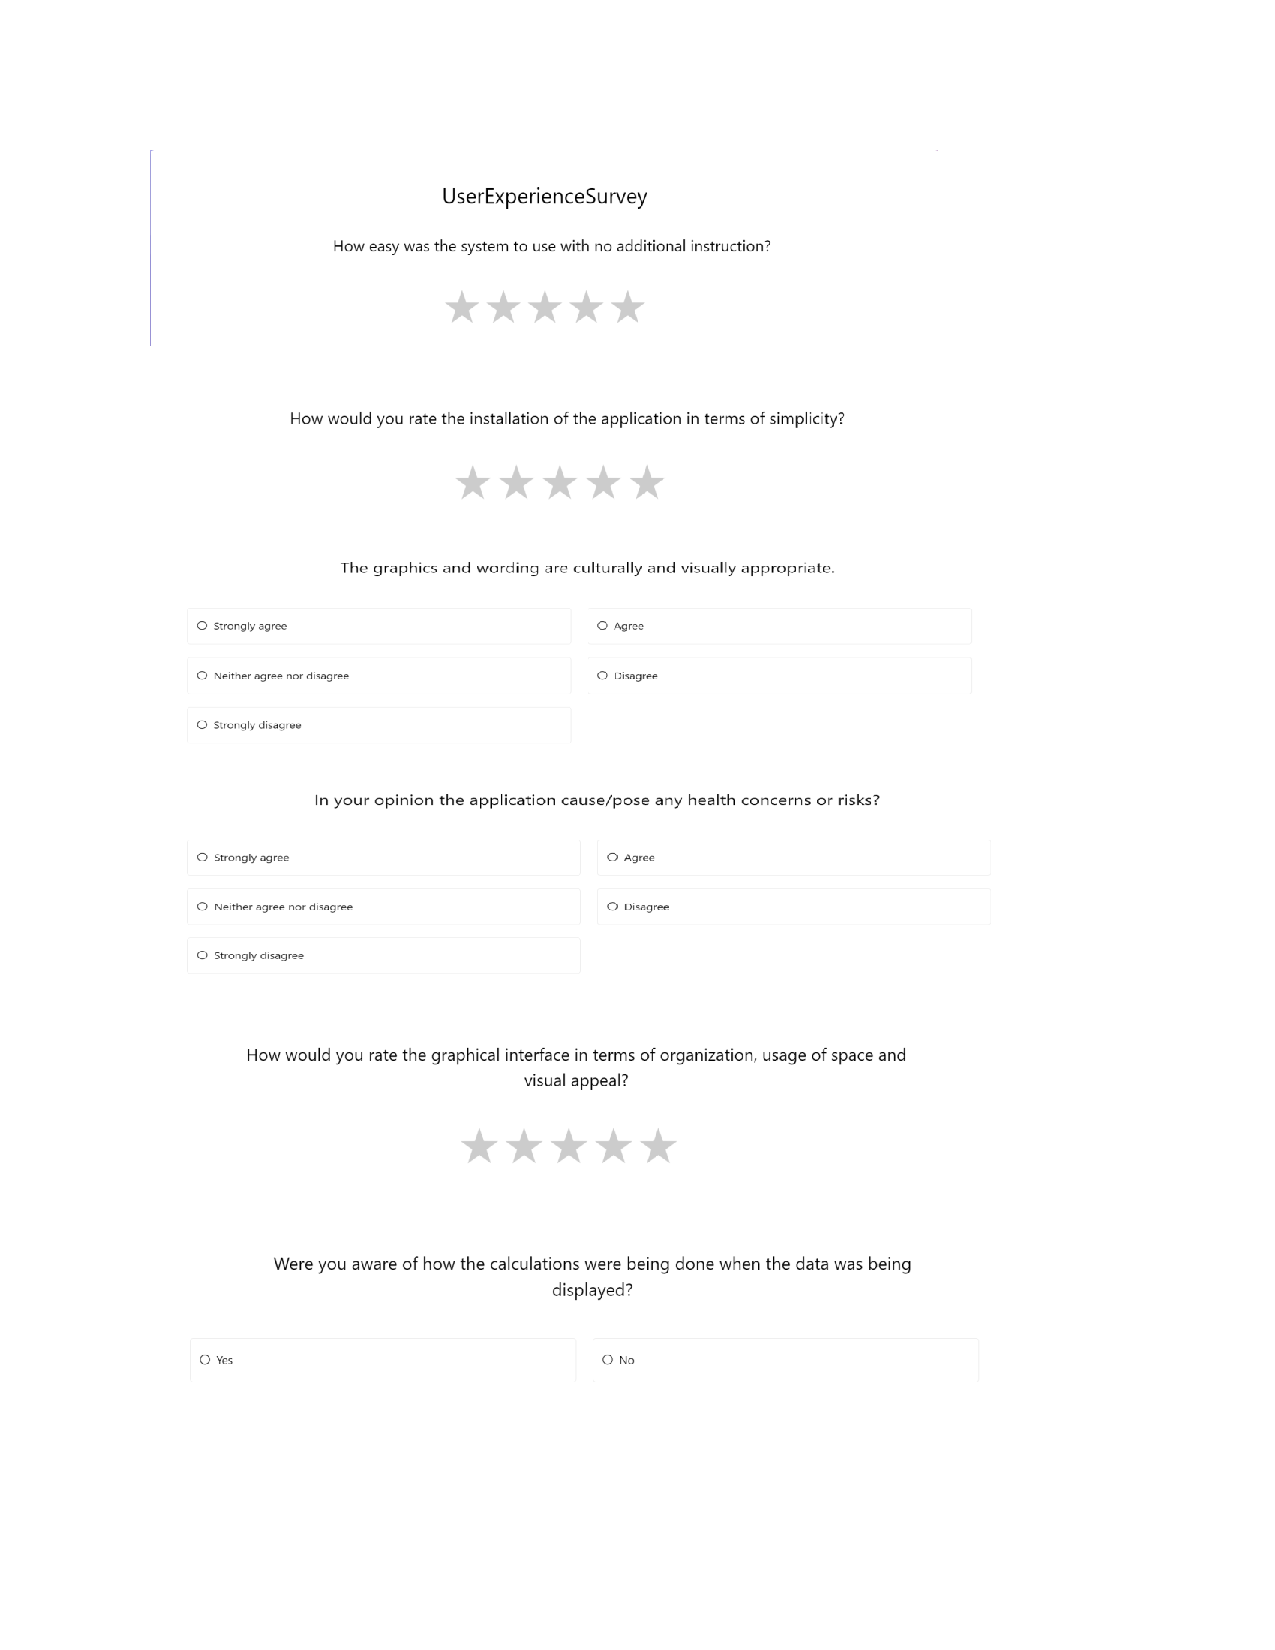
\includegraphics[width=1\textwidth]{UserExperienceSurvey.pdf}
\end{figure}


\newpage{}
\section*{Appendix --- Reflection}

The information in this section will be used to evaluate the team members on the
graduate attribute of Lifelong Learning.  Please answer the following questions:

\begin{enumerate}
  \item 
  \item 
\end{enumerate}

\end{document}